\documentclass[xcolor=pdftex,romanian,colorlinks]{beamer}
%\documentclass[xcolor=pdftex,handout,romanian,colorlinks]{beamer}

\usepackage[export]{adjustbox}
\usepackage{../sty/tslides}
\usepackage[all]{xy}
\usepackage{pgfplots}
\usepackage{flowchart}
\usepackage{todonotes}
\usetikzlibrary{arrows,positioning,calc}
\lstset{language=Haskell}
\lstset{escapeinside={(*@}{@*)}}
\PrerenderUnicode{ăĂîÎȘșȚțâÂ}
\usepackage{amsmath}

%\usepackage{xcolor}
%\definecolor{IntensColor}{HTML}{2E86C1}
%\definecolor{StateTransition}{HTML}{D6EAF8}
%\definecolor{MedianLightOrange}{RGB}{216,178,92}
%\definecolor{Orchid}{HTML}{8E44AD}
%\definecolor{True}{HTML}{229954}
%\definecolor{False}{HTML}{CB4335}


\usepackage{proof}
\usepackage{multirow}
\usepackage{alltt}
\usepackage{mathpartir}
\usepackage{ulem}

\newcommand{\structured}[1]{#1}

\definecolor{IntensColor}{HTML}{2E86C1}
\definecolor{StateTransition}{HTML}{D6EAF8}
\definecolor{MedianLightOrange}{RGB}{216,178,92}
\definecolor{Orchid}{HTML}{8E44AD}
\definecolor{True}{HTML}{229954}
\definecolor{False}{HTML}{CB4335}

\newcommand{\cin}[1]{{\color{cobalt} #1}}
\newcommand{\sel}[1]{{\color{Orchid} #1}}

\newcommand{\intens}[1] {{\color{IntensColor} #1}}
\newcommand{\exe}[1] {{\color{True} #1}}

\newcommand{\la}{\lambda}

\setlength{\leftmargini}{0pt}

\newcommand{\app}[2]{#1\, #2}
\newcommand{\abs}[2]{\lambda #1.\,#2}

\newcommand{\type}[2]{{\color{True}#1\hspace{-.05cm}:}\,{\color{Orchid}#2}}

\newcommand{\sub}[3]{#1\langle#2/#3\rangle}
\newcommand{\subt}[3]{#1[#2/#3]}
\newcommand{\equiva}{=_\alpha}

\newcommand{\trueL}{\mathbf{T}}
\newcommand{\falseL}{\mathbf{F}}
\newcommand{\notL}{\mathbf{not}}
\newcommand{\andL}{\mathbf{and}}
\newcommand{\orL}{\mathbf{or}}
\newcommand{\ifL}{\mathbf{if}}
\newcommand{\boolL}{\mathbf{bool}}

\newcommand{\maybeL}{\mathbf{maybe}}
\newcommand{\nothingL}{\mathbf{Nothing}}
\newcommand{\justL}{\mathbf{Just}}
\newcommand{\Maybe}[1]{\mathop{\mathbf{Maybe}}{#1}}

\newcommand{\foldrL}{\mathbf{foldr}}
\newcommand{\nilL}{\mathbf{Nil}}
\newcommand{\consL}{\mathbf{Cons}}
\newcommand{\ListL}[1]{\mathop{\mathbf{List}}{#1}}

\newcommand{\unpairL}{\mathbf{uncons}}
\newcommand{\pairL}{\mathbf{Pair}}
\newcommand{\firstL}{\mathbf{first}}
\newcommand{\secondL}{\mathbf{second}}
\newcommand{\Pair}[2]{\mathop{\mathop{\mathbf{Pair}}{#1}}{#2}}

\newcommand{\succL}{\mathbf{Succ}}
\newcommand{\zeroL}{\mathbf{Zero}}
\newcommand{\iterateL}{\mathbf{iterate}}
\newcommand{\addL}{\mathbf{add}}
\newcommand{\mulL}{\mathbf{mul}}
\newcommand{\expL}{\mathbf{exp}}
\newcommand{\isZero}{\mathbf{isZero}}
\newcommand{\pred}{\mathbf{pred}}
\newcommand{\factL}{\mathbf{fact}}

\newcommand{\BoolT}{\ensuremath{\texttt{Bool}}}
%\newcommand{\BoolT}{\ensuremath{\texttt{Bool}}}
\newcommand{\ifT}[3]{\mathrm{if}\ #1\ \mathrm{then}\ #2\ \mathrm{else}\ #3}

\newcommand{\UnitT}{\ensuremath{\texttt{Unit}}}
\newcommand{\unit}{\mathrm{unit}}

\newcommand{\VoidT}{\ensuremath{\texttt{Void}}}
\newcommand{\void}{\mathrm{void}}


\newcommand{\ProductT}[2]{#1 \times #2}
\newcommand{\PairL}[2]{\langle #1,#2\rangle}
\newcommand{\ProjOne}[1]{fst\ #1}
\newcommand{\ProjTwo}[1]{snd\ #1}

\newcommand{\SumT}[2]{#1 + #2}
\newcommand{\Left}[1]{\mathrm{Left}\ #1}
\newcommand{\Right}[1]{\mathrm{Right}\ #1}
\newcommand{\Case}[3]{\mathrm{case}\ #1\ \mathrm{of}\ #2\ ;\ #3}

%----------------------------------------------

\newcommand{\SSnot}{\terminal{not}}

\newcommand{\Sand}{\terminal{and}}
\newcommand{\Sor}{\terminal{or}}
\newcommand{\Splus}{\terminal{+}}
\newcommand{\Smul}{\terminal{*}}
\newcommand{\Ssucc}{\terminal{S}}
\newcommand{\Spow}{\terminal{pow}}
\newcommand{\Spred}{\terminal{pred}}
\newcommand{\Seq}{\terminal{eq}}
\newcommand{\Sneq}{\terminal{neq}}

\newcommand{\SisZero}{\terminal{isZero}}
\newcommand{\Slte}{\terminal{<=}}
\newcommand{\Sgte}{\terminal{>=}}
\newcommand{\Slt}{\terminal{<}}
\newcommand{\Sgt}{\terminal{>}}
\newcommand{\Spair}{\terminal{pair}}
\newcommand{\Sfst}{\terminal{fst}}
\newcommand{\Ssnd}{\terminal{snd}}
\newcommand{\Sminus}{\terminal{-}}

\newcommand{\Snull}{\terminal{null}}
\newcommand{\Scons}{\terminal{cons}}
%\newcommand{\c sead}{\terminal{head}}
\newcommand{\SisNull}{\terminal{?null}}
\newcommand{\Stail}{\terminal{tail}}
\newcommand{\Ssum}{\terminal{sum}}
\newcommand{\Sfoldr}{\terminal{foldr}}
\newcommand{\Smap}{\terminal{map}}
\newcommand{\Sfilter}{\terminal{filter}}

\newcommand{\const}[1]{\triangleright {\color{False} #1}}

\newcommand{\egf}[1]{\stackrel{\cdot}{=}_{#1}}

\newcommand{\Conf}[2]{\ensuremath{\langle #1\ ,\ #2\rangle}}
\newcommand{\plus}[1] {{\color{True} #1}}
\newcommand{\te}[1]{\mbox{\texttt{#1}}}

\newcommand{\vexp}{\ensuremath{\mathbb{E}}}
\newcommand{\bexp}{\ensuremath{\mathbb{B}}}
\newcommand{\cmd}{\ensuremath{\mathbb{C}}}

\definecolor{section-color}{HTML}{23373b} %mDarkTeal
%\AtBeginSection[]{
%  \begin{frame}
%  \vfill
%  \centering
%  \begin{beamercolorbox}[sep=8pt,center,shadow=true,rounded=true]{title}
%    \usebeamerfont{title}\insertsectionhead\par%
%  \end{beamercolorbox}
%  \vfill
%  \end{frame}
%}



\title[FLP]{Fundamentele limbajelor de programare}
\subtitle{C03}
\date{}


\begin{document}
\begin{frame}
  \titlepage
\end{frame}

\setlength{\leftmargini}{12pt}

%================================================
\section{\color{section-color} Lambda calcul - $\beta$-reducții}
%================================================

%------------------------------------------------
\begin{frame}[fragile]{$\beta$-reducții}

\alert{Convenție.} Spunem că doi termeni sunt egali, notat \intens{$M = N$},\\ dacă sunt $\alpha$-echivalenți.

\begin{itemize}
	\item \alert{$\beta$-reducție} = procesul de a evalua lambda termeni prin "pasarea de argumente funcțiilor"

	\item \alert{$\beta$-redex} = un termen de forma \intens{$\app{(\abs{x}{M})}{N}$}

	\item \alert{redusul} unui redex \intens{$\app{(\abs{x}{M})}{N}$} este \intens{$\subt{M}{N}{x}$}
	
	\item reducem lambda termeni prin găsirea unui subtermen care este redex, și apoi înlocuirea acelui redex cu redusul său
	
	\item repetăm acest proces de câte ori putem, până nu mai sunt redex-uri
	
	\item \alert{formă normală} = un lambda termen fără redex-uri
\end{itemize}
\end{frame}

%------------------------------------------------
\begin{frame}[fragile]{$\beta$-reducții}

Un pas de $\beta$-reducție \intens{$\rightarrow_\beta$}  este cea mai mică relație pe lambda termeni care satisface regulile:

\begin{center}
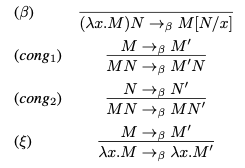
\includegraphics[scale=.6]{images/beta-reduct}
\end{center}

\end{frame}

%------------------------------------------------
\begin{frame}[fragile]{$\beta$-reducții}

La fiecare pas, subliniem redexul ales în procesul de $\beta$-reducție.

\begin{center}
\begin{tabular}{rcl}
$\app{(\abs{x}{y})}{(\underline{\app{(\abs{z}{\app{zz}})}{(\abs{w}{w})}})}$ & $\rightarrow_\beta$ & $\app{(\abs{x}{y})}{( \subt{(\app{z}{z})}{\abs{w}{w}}{z} )}$ \\ 
& $\equiv$ & $\app{(\abs{x}{y})}{( \app{(\subt{z}{\abs{w}{w}}{z})}{(\subt{z}{\abs{w}{w}}{z} )}}$ \\
& $\equiv$ & $\app{(\abs{x}{y})}{(\underline{\app{(\abs{w}{w})}{(\abs{w}{w})}})}$ \\
& $\rightarrow_\beta$ & $\underline{\app{(\abs{x}{y})}{(\abs{w}{w})}}$ \\
& $\rightarrow_\beta$ & $y$ \\
\end{tabular}
\end{center}

Ultimul termen nu mai are redex-uri, deci este în formă normală.

\end{frame}

%------------------------------------------------
\begin{frame}[fragile]{$\beta$-reducții}

\begin{center}
\begin{tabular}{rcl}
$\app{(\abs{x}{y})}{(\underline{\app{(\abs{z}{\app{zz}})}{(\abs{w}{w})}})}$ & $\rightarrow_\beta$ &  $\app{(\abs{x}{y})}{(\underline{\app{(\abs{w}{w})}{(\abs{w}{w})}})}$ \\
& $\rightarrow_\beta$ & $\underline{\app{(\abs{x}{y})}{(\abs{w}{w})}}$ \\
& $\rightarrow_\beta$ & $y$ \\
\end{tabular}
\end{center}

\begin{center}
\begin{tabular}{rcl}
$\underline{\app{(\abs{x}{y})}{(\app{(\abs{z}{\app{zz}})}{(\abs{w}{w})})}}$ & $\rightarrow_\beta$ & $\subt{y}{\app{(\abs{z}{\app{zz}})}{(\abs{w}{w})}}{x}$ \\ 
& $\equiv$ & $y$ \\
\end{tabular}
\end{center}

Observăm că:
\begin{itemize}
	\item reducerea unui redex poate crea noi redex-uri
	\item reducerea unui redex poate șterge alte redex-uri
	\item numărul de pași necesari până a atinge o formă normală poate varia, în funcție de ordinea în care sunt reduse redex-urile
	\item rezultatul final pare că nu a depins de alegerea redex-urilor 
\end{itemize}

\end{frame}


%------------------------------------------------
\begin{frame}[fragile]{$\beta$-formă normală}

Totuși, există lambda termeni care nu pot fi reduși la o $\beta$-formă normală (evaluarea nu se termină).

\begin{center}
\begin{tabular}{rcl}
$\underline{\app{(\abs{x}{\app{x}{x}})}{(\abs{x}{\app{x}{x}})}}$ & $\rightarrow_\beta$ & $\app{(\abs{x}{\app{x}{x}})}{(\abs{x}{\app{x}{x}})}$ \\
& $\rightarrow_\beta$ & $\ldots$ \\
\end{tabular}
\end{center}

Observați că lungimea unui termen nu trebuie să scadă în procesul de $\beta$-reducție; poate crește sau rămâne neschimbat.
\end{frame}

%------------------------------------------------
\begin{frame}[fragile]{$\beta$-formă normală}

Există lambda termeni care deși pot fi reduși la o formă normală, pot să nu o atingă niciodată.

{\footnotesize
\begin{center}
\begin{tabular}{rcl} 
$\app{\underline{\app{(\abs{xy}{y})}{(\app{(\abs{x}{\app{x}{x}})}{(\abs{x}{\app{x}{x}})})}}}{(\abs{z}{z})}$ & $\rightarrow_\beta$ & $\underline{\app{(\abs{y}{y})}{(\abs{x}{x})}}$ \\
&$\rightarrow_\beta$ & $\abs{x}{x}$ \\[.4cm] 
$\app{\app{(\abs{xy}{y})}{(\underline{\app{(\abs{x}{\app{x}{x}})}{(\abs{x}{\app{x}{x}})})}}}{(\abs{z}{z})}$ & $\rightarrow_\beta$ &  $\app{\app{(\abs{xy}{y})}{(\app{(\abs{x}{\app{x}{x}})}{(\abs{x}{\app{x}{x})})}}}{(\abs{z}{z})}$ \\
\end{tabular}
\end{center}
}

Contează \alert{strategia de evaluare.}
\end{frame}

%------------------------------------------------
\begin{frame}[fragile]{$\beta$-formă normală}

Notăm cu \intens{$M \twoheadrightarrow_\beta M'$} faptul că $M$ poate fi $\beta$-redus până la $M'$ în $0$ sau mai mulți pași  (închiderea reflexivă și tranzitivă a relației $\rightarrow_\beta$).

\medskip
$M$ este \intens{slab normalizabil} \textit{(weakly normalising)} dacă există $N$ în formă normală astfel încât $M \twoheadrightarrow_\beta N$.

\medskip
$M$ este \intens{puternic normalizabil} \textit{(strong normalising)} dacă nu există reduceri infinite care încep din $M$.

\medskip
Orice termen puternic normalizabil este și slab normalizabil.

\medskip
\begin{example}

\smallskip
$\app{(\abs{x}{y})}{(\app{(\abs{z}{\app{zz}})}{(\abs{w}{w})})}$ este {\color{True} puternic normalizabil}.

\smallskip
$\app{\app{(\abs{xy}{y})}{(\app{(\abs{x}{\app{x}{x}})}{(\abs{x}{\app{x}{x}})})}}{(\abs{z}{z})}$ este {\color{True} slab normalizabil}, \\ dar {\color{False} nu puternic normalizabil}.



\end{example}
\end{frame}


%------------------------------------------------
\begin{frame}[fragile]{Confluența $\beta$-reducției}

\bigskip
\alert{Teorema Church-Rosser.}
Dac\u a $M \twoheadrightarrow_\beta M_1$ și $M \twoheadrightarrow_\beta M_2$ atunci exist\u a $M'$ astfel încât $M_1 \twoheadrightarrow_\beta M'$ și $M_2\twoheadrightarrow_\beta M'$.

\vspace{-.4cm}
\begin{figure}[h]
  \centering
  \begin{tikzpicture}	
  	\node(t) at (0,2) {$M$}; 
	\node(t1) at (-2,1) {$M_1$};
   	\node(t2) at (2,1) {$M_2$};
	\node (u) at (0,0) {$M'$};
	\draw [->>]  (t) -- (t1) ;
	\draw [->>]  (t) -- (t2) ;
	\draw [->>, dashed]  (t1) -- (u) ;
	\draw [->>, dashed]  (t2) -- (u) ;
   \end{tikzpicture}
\end{figure} 

\alert{Consecință.} Un lambda termen are cel mult o $\beta$-formă normală (modulo $\alpha$-echivalență).
\end{frame}

%------------------------------------------------
\begin{frame}[fragile]{Exerciții}

\textbf{\intens{Exercițiu.}} 
Verificați dacă termenii de mai jos pot fi aduși la o $\beta$-formă normală:
\begin{enumerate}
	\item \alert{$\app{(\abs{x}{x})}{M}$} \onslide<2->{\hfill {\color{True} Corect: $M$}}

	\smallskip
	\item \alert{$\app{\app{(\abs{xy}{x})}{M}}{N}$} \onslide<2->{\hfill {\color{True} Corect: $M$}}

	\smallskip
	\item \alert{$\app{(\abs{x}{\app{x}{x}})}{(\abs{y}{\app{\app{y}{y}}{y}})}$} \onslide<2->{\hfill {\color{True} Corect: $\app{\app{(\abs{y}{\app{\app{y}{y}}{y}})}{(\abs{y}{\app{\app{y}{y}}{y}})}}{(\abs{y}{\app{\app{y}{y}}{y}})}\ldots$}}
\end{enumerate}

\end{frame}


%================================================
\section{\color{section-color} Strategii de evaluare}
%================================================

%------------------------------------------------
\begin{frame}[fragile]{Strategii de evaluare}

De cele mai multe ori, există mai mulți pași de $\beta$-reducție care pot fi aplicați unui termen. Cum alegem ordinea? Contează ordinea?

\medskip  
O \alert{strategie de evaluare} ne spune în ce ordine să facem pașii de reducție.


\medskip  
Lambda calculul nu specifică o strategie de evaluare, fiind \alert{nedeterminist}. O strategie de evaluare este necesară în limbaje de programare reale pentru a rezolva nedeterminismul.

\end{frame}

%------------------------------------------------
\begin{frame}[fragile]{Strategia normală (normal order)}

\intens{Strategia normală = \textit{leftmost-outermost}}\\
(alegem redex-ul cel mai din stânga și apoi cel mai din exterior)

\begin{itemize}
	\item dacă $M_1$ și $M_2$ sunt redex-uri  și $M_1$ este un subtermen al lui $M_2$, atunci $M_1$ {\color{False} nu} va fi următorul redex ales
	\item printre redex-urile care nu sunt subtermeni ai altor redex-uri (și sunt incomparabili față de relația de subtermen), îl alegem pe cel mai din stânga.
\end{itemize}

\alert{Dacă un termen are o formă normală, atunci strategia normală va converge la ea}.

{\footnotesize
\begin{center}
\begin{tabular}{rcl} 
$\app{\underline{\app{(\abs{xy}{y})}{(\app{(\abs{x}{\app{x}{x}})}{(\abs{x}{\app{x}{x}})})}}}{(\abs{z}{z})}$ & $\rightarrow_\beta$ & $\underline{\app{(\abs{y}{y})}{(\abs{x}{x})}}$ \\
&$\rightarrow_\beta$ & $\abs{x}{x}$ %\\[.4cm] 
%$\app{\app{(\abs{xy}{y})}{(\underline{\app{(\abs{x}{\app{x}{x}})}{(\abs{x}{\app{x}{x}})})}}}{(\abs{z}{z})}$ & $\rightarrow_\beta$ &  $\app{\app{(\abs{xy}{y})}{(\app{(\abs{x}{\app{x}{x}})}{(\abs{x}{\app{x}{x})})}}}{(\abs{z}{z})}$ \\
\end{tabular}
\end{center}
}

\end{frame}


%------------------------------------------------
\begin{frame}[fragile]{Strategia aplicativă (applicative order)}

\intens{Strategia aplicativă = \textit{leftmost-innermost}} \\
(alegem redex-ul  cel mai din stânga și apoi cel mai din interior)

\begin{itemize}
	\item dacă $M_1$ și $M_2$ sunt redex-uri  și $M_1$ este un subtermen al lui $M_2$, atunci $M_2$ {\color{False} nu} va fi următorul redex ales
	\item printre redex-urile care nu sunt subtermeni ai altor redex-uri (și sunt incomparabili față de relația de subtermen), îl alegem pe cel mai din stânga.
\end{itemize}

{\footnotesize
\begin{center}
\begin{tabular}{rcl} 
%$\app{\underline{\app{(\abs{xy}{y})}{(\app{(\abs{x}{\app{x}{x}})}{(\abs{x}{\app{x}{x}})})}}}{(\abs{z}{z})}$ & $\rightarrow_\beta$ & $\underline{\app{(\abs{y}{y})}{(\abs{x}{x})}}$ \\
%&$\rightarrow_\beta$ & $\abs{x}{x}$ \\[.4cm] 
$\app{\app{(\abs{xy}{y})}{(\underline{\app{(\abs{x}{\app{x}{x}})}{(\abs{x}{\app{x}{x}})})}}}{(\abs{z}{z})}$ & $\rightarrow_\beta$ &  $\app{\app{(\abs{xy}{y})}{(\app{(\abs{x}{\app{x}{x}})}{(\abs{x}{\app{x}{x})})}}}{(\abs{z}{z})}$ \\
\end{tabular}
\end{center}
}

\end{frame}

%------------------------------------------------
\begin{frame}[fragile]{Strategii în programare funcțională}

În limbaje de programare funcțională, în general, reducerile din corpul unei $\lambda$-abstractizări nu sunt efectuate (deși anumite compilatoare optimizate pot face astfel de reduceri în unele cazuri).

\medskip
\intens{Strategia \textit{call-by-name} (CBN)} = strategia normală fără a face reduceri în corpul unei $\lambda$-abstractizări

\medskip
\intens{Strategia \textit{call-by-value} (CBV)} = strategia aplicativă fără a face reduceri în corpul unei $\lambda$-abstractizări

\medskip
Majoritatea limbajelor de programare funcțională folosesc CBV, excepție făcând Haskell.

\end{frame}

%------------------------------------------------
\begin{frame}[fragile]{CBN vs CBV}

O \intens{valoare} este un $\lambda$-term pentru care nu există $\beta$-reducții date de strategia de evaluare considerată.

De exemplu, {\color{True} $\abs{x}{x}$} este mereu o valoare, dar {\color{False} $\app{(\abs{x}{x})}{1}$} nu este.

Sub \intens{CBV}, funcțille pot fi apelate doar prin valori (argumentele trebuie să fie complet evaluate). Astfel, putem face $\beta$-reducția \intens{$\app{(\abs{x}{M})}{N} \twoheadrightarrow_\beta \subt{M}{N}{x}$} doar dacă $N$ este valoare.

Sub \intens{CBN}, amânăm evaluarea argumentelor cât mai mult posibil, făcând reducții de la stânga la dreapta în expresie. Aceasta este strategia folosită în Haskell. 

CBN este o formă de evaluare leneșă \textit{(lazy evaluation)}: argumentele funcțiilor sunt evaluate doar când sunt necesare.

\end{frame}

%------------------------------------------------
\begin{frame}[fragile]{CBN vs CBV}

\begin{example}
\smallskip
Considerăm $3$ și $succ$ primitive.

\intens{Strategia CBV:}

\vspace{-.4cm}
\begin{center}
\begin{tabular}{rcl}
$\app{(\abs{x}{\app{succ}{x}})}{(\app{(\abs{y}{\app{succ}{y}})}{3})}$ & $\twoheadrightarrow_\beta$ & $\app{(\abs{x}{\app{succ}{x}})}{(\app{succ}{3})}$ \\
& $\rightarrow$ & $\app{(\abs{x}{\app{succ}{x}})}{4}$ \\
& $\twoheadrightarrow_\beta$ & $\app{succ}{4}$ \\
& $\rightarrow$ &  $5$
\end{tabular}
\end{center} 

\intens{Strategia CBN:}
\vspace{-.4cm}
\begin{center}
\begin{tabular}{rcl}
$\app{(\abs{x}{\app{succ}{x}})}{(\app{(\abs{y}{\app{succ}{y}})}{3})}$ & $\twoheadrightarrow_\beta$ & $\app{succ}{(\app{(\abs{y}{\app{succ}{y}})}{3})}$ \\
& $\twoheadrightarrow_\beta$ & $\app{succ}{(\app{succ}{3})}$ \\
& $\rightarrow$ & $\app{succ}{4}$ \\
& $\rightarrow$ & $5$ \\
\end{tabular}
\end{center} 
\end{example}

\end{frame}

%%================================================
%\section{\color{section-color} Expresivitatea $\lambda$-calculului}
%%================================================
%
%\begin{frame}{Expresivitatea $\lambda$-calculului}
%
%Deși lambda calculul constă doar în $\lambda$-termeni, putem reprezenta și manipula tipuri de date comune.
%
%Vom vedea cum putem reprezenta:
%\begin{itemize}
%	\item valori booleene
%	\item numere naturale
%	\item liste
%%	\item maybe 
%\end{itemize}
%\end{frame}
%
%%------------------------------------------------
%\begin{frame}{Booleeni}
%
%Vrem să definim $\lambda$-termeni care să reprezinte constantele booleene.
%
%Sunt mai multe modalități, una dintre ele fiind:
%
%\begin{itemize}
%	\item \intens{$\trueL \triangleq \abs{xy}{x}$}  \hfill (dintre cele două alternative o alege pe prima)
%	\item \intens{$\falseL \triangleq \abs{xy}{y}$} \hfill (dintre cele două alternative o alege pe a doua)
%\end{itemize}
%
%\end{frame}
%
%%------------------------------------------------
%\begin{frame}{Booleeni}
%
%\begin{center}
% \intens{$\trueL \triangleq \abs{xy}{x}$} \hspace{1cm} \intens{$\falseL \triangleq \abs{xy}{y}$}
%\end{center}
%
%\vspace{-.2cm}
%Acum am vrea să definim un test condiționat $\ifL$. 
%
%Am vrea ca $\ifL$ să ia trei argumente $b,t,f$, unde $b$ este o valoare booleană, iar $t,f$ sunt $\lambda$-termeni oarecare. 
%
%Funcția ar trebui să returneze $t$ dacă $b = true$ și $f$ dacă $b = false$
%\begin{center}
%$\ifL = \abs{btf}{\left\{ \begin{array}{ll}
%         t, & \mbox{if $b = true$},\\
%        f, & \mbox{if $b = false$}.\end{array} \right.}$
%\end{center}
%
%Deoarece $\app{\app{\trueL}{t}}{f} \twoheadrightarrow_\beta t$ și $\app{\app{\falseL}{t}}{f} \twoheadrightarrow_\beta f$, $\ifL$ trebuie doar să aplice argumentul său boolean celorlalte argumente:
%\begin{center}
%\intens{$\ifL \triangleq \abs{btf}{\app{\app{b}{t}}{f}}$}
%\end{center}
%\end{frame}
%
%%------------------------------------------------
%\begin{frame}{Booleeni}
%
%\begin{center}
% \intens{$\trueL \triangleq \abs{xy}{x}$} \hspace{1cm} \intens{$\falseL \triangleq \abs{xy}{y}$ \hspace{1cm} $\ifL \triangleq \abs{btf}{\app{\app{b}{t}}{f}}$}
%\end{center}
%
%\vspace{-.2cm}
%Celelalte operații booleene pot fi definite folosind $\ifL$:
%
%\begin{center}
%\begin{tabular}{rcl}
%\intens{$\andL$} & \hspace{-.3cm} \intens{$\triangleq$} & \hspace{-.3cm} \intens{$\abs{b_1b_2}{\app{\app{\app{\ifL}{b_1}}{b_2}}{\falseL}}$} \\
%\intens{$\orL$} & \hspace{-.3cm} \intens{$\triangleq$} & \hspace{-.3cm} \intens{$\abs{b_1b_2}{\app{\app{\app{\ifL}{b_1}}{\trueL}}{b_2}}$} \\
%\intens{$\notL$} & \hspace{-.3cm} \intens{$\triangleq$} & \hspace{-.3cm} \intens{$\abs{b_1}{\app{\app{\app{\ifL}{b_1}}{\falseL}}{\trueL}}$} \\
%\end{tabular}
%\end{center}
%
%Observați că aceste operații lucrează corect doar dacă primesc ca valori booleene. 
%
%Nu există nicio garanție să se comporte rezonabil pe orice alți $\lambda$-termeni.
%
%Folosind lambda calcul fără tipuri, avem \intens{\textit{garbage in, garbage out}}.
%\end{frame}
%
%%------------------------------------------------
%\begin{frame}{Booleeni}
%
%\begin{center}
% \intens{$\trueL \triangleq \abs{xy}{x}$} \hspace{.4cm} \intens{$\falseL \triangleq \abs{xy}{y}$ \hspace{.4cm} $\ifL \triangleq \abs{btf}{\app{\app{b}{t}}{f}}$}
% 
% \begin{tabular}{rcl}
%\intens{$\andL$} & \hspace{-.3cm} \intens{$\triangleq$} & \hspace{-.3cm} \intens{$\abs{b_1b_2}{\app{\app{\app{\ifL}{b_1}}{b_2}}{\falseL}}$} \\
%\intens{$\orL$} & \hspace{-.3cm} \intens{$\triangleq$} & \hspace{-.3cm} \intens{$\abs{b_1b_2}{\app{\app{\app{\ifL}{b_1}}{\trueL}}{b_2}}$} \\
%\intens{$\notL$} & \hspace{-.3cm} \intens{$\triangleq$} & \hspace{-.3cm} \intens{$\abs{b_1}{\app{\app{\app{\ifL}{b_1}}{\falseL}}{\trueL}}$} \\
%\end{tabular}
%
%\end{center}
%
%
%\intens{\textbf{Exercițiu.}} Aduceți la o formă normală următorii termenii:
%\begin{itemize}
%	\item \alert{$\app{\app{\andL}{\trueL}{\falseL}}$}
%	\item \alert{$\app{\app{\orL}{\falseL}{\trueL}}$}
%	\item \alert{$\app{\notL}{\trueL} $}
%\end{itemize}
%\end{frame}
%
%%------------------------------------------------
%\begin{frame}{Booleeni}
%
%\begin{center}
% \intens{$\trueL \triangleq \abs{xy}{x}$} \hspace{.4cm} \intens{$\falseL \triangleq \abs{xy}{y}$ \hspace{.4cm} $\ifL \triangleq \abs{btf}{\app{\app{b}{t}}{f}}$}
% 
% \begin{tabular}{rcl}
%\intens{$\andL$} & \hspace{-.3cm} \intens{$\triangleq$} & \hspace{-.3cm} \intens{$\abs{b_1b_2}{\app{\app{\app{\ifL}{b_1}}{b_2}}{\falseL}}$} \\
%\intens{$\orL$} & \hspace{-.3cm} \intens{$\triangleq$} & \hspace{-.3cm} \intens{$\abs{b_1b_2}{\app{\app{\app{\ifL}{b_1}}{\trueL}}{b_2}}$} \\
%\intens{$\notL$} & \hspace{-.3cm} \intens{$\triangleq$} & \hspace{-.3cm} \intens{$\abs{b_1}{\app{\app{\app{\ifL}{b_1}}{\falseL}}{\trueL}}$} \\
%\end{tabular}
%
%\end{center}
%
%\textbf{Soluții:}
%
%$\app{\app{\andL}{\trueL}{\falseL}} = \app{\app{(\abs{b_1b_2}{\app{\app{\app{\ifL}{b_1}}{b_2}}{\falseL}})}{\trueL}{\falseL}} \twoheadrightarrow_\beta \app{\app{\app{\ifL}{\trueL}}{\falseL}}{\falseL} = \app{\app{\app{(\abs{btf}{\app{\app{b}{t}}{f}})}{\trueL}}{\falseL}}{\falseL}$\\
%\hspace{1.2cm} $\twoheadrightarrow_\beta  \app{\app{\trueL}{\falseL}}{\falseL} = \app{\app{(\abs{xy}{x})}{\falseL}}{\falseL} \twoheadrightarrow_\beta \falseL$
%
%$\app{\app{\orL}{\falseL}{\trueL}} = \app{\app{(\abs{b_1b_2}{\app{\app{\app{\ifL}{b_1}}{\trueL}}{b_2}})}{\falseL}{\trueL}} \twoheadrightarrow_\beta \app{\app{\app{\ifL}{\falseL}}{\trueL}}{\trueL} = \app{\app{\app{(\abs{btf}{\app{\app{b}{t}}{f}})}{\falseL}}{\trueL}}{\trueL}$ \\
%\hspace{1.2cm} $\twoheadrightarrow_\beta \app{\app{\falseL}{\trueL}}{\trueL} =  \app{\app{(\abs{xy}{y})}{\trueL}}{\trueL} \twoheadrightarrow_\beta  \trueL$
%
%$\app{\notL}{\trueL} = \app{(\abs{b_1}{\app{\app{\app{\ifL}{b_1}}{\falseL}}{\trueL}})}{\trueL} \twoheadrightarrow_\beta \app{\app{\app{\ifL}{\trueL}}{\falseL}}{\trueL} = \app{\app{\app{(\abs{btf}{\app{\app{b}{t}}{f}})}{\trueL}}{\falseL}}{\trueL}$ \\
%\hspace{1.2cm} $\twoheadrightarrow_\beta \app{\app{\trueL}{\falseL}}{\trueL} = \app{\app{(\abs{xy}{x})}{\falseL}}{\trueL} \twoheadrightarrow_\beta \falseL $
%
%\end{frame}
%
%%------------------------------------------------
%\begin{frame}{Numere naturale}
%
%Vom reprezenta numerele naturale $\mathbb{N}$ folosind \alert{numeralii Church}.
%
%Numeralul Church pentru numărul $n \in \mathbb{N}$ este notat \intens{$\overline{n}$}.
%
%Numeralul Church $\overline{n}$ este $\lambda$-termenul \intens{$\abs{fx}{\app{f^n}{x}}$}, unde $f^n$ reprezintă compunerea lui $f$ cu ea însăși de $n$ ori:
%
%\begin{center}
%\begin{tabular}{rcccl}
%\intens{$\overline{0}$} & $\triangleq$ & $\abs{fx}{\app{f^0}{x}}$ & $=$ & $\abs{fx}{x}$ \\
%\intens{$\overline{1}$} & $\triangleq$ & $\abs{fx}{\app{f^1}{x}}$ & $=$ & $\abs{fx}{\app{f}{x}}$ \\
%\intens{$\overline{2}$} & $\triangleq$ & $\abs{fx}{\app{f^2}{x}}$ & $=$ & $\abs{fx}{\app{f}{(\app{f}{x})}}$ \\
%\intens{$\overline{3}$} & $\triangleq$ & $\abs{fx}{\app{f^3}{x}}$ & $=$ & $\abs{fx}{\app{f}{(\app{f}{(\app{f}{x})})}}$ \\
%& $\vdots$ && \\
%\intens{$\overline{n}$} & $\triangleq$ & $\abs{fx}{\app{f^n}{x}}$ & $=$ & $\abs{fx}{\underbrace{f(f(\ldots(f}_{n}\,x)\ldots))}$ \\
%\end{tabular}
%\end{center}
%
%
%\end{frame}
%
%%------------------------------------------------
%\begin{frame}{Numere naturale}
%
%\begin{center}
%\intens{$\overline{n} \triangleq \abs{fx}{\app{f^n}{x}}$}
%\end{center}
%
%\vspace{-.4cm}
%Acum putem defini funcția \alert{succesor} prin
%\vspace{-.2cm}
%\begin{center}
%\intens{$\succL \triangleq \abs{nfx}{\app{f}{(\app{\app{n}{f}}{x})}}$}
%\end{center}
%
%\vspace{-.2cm}
%Observați că $\succL$ pe argumentul $\overline{n}$ returnează o funcție care primește ca argument o funcție $f$, îi aplică $\overline{n}$ pentru a obține compunerea de $n$ ori a lui $f$ cu ea însăși, apoi aplică iar $f$ pentru a obține compunerea de $n+1$ ori a lui $f$ cu ea însăși.
%
%\vspace{-.2cm}
%\begin{center}
%\begin{tabular}{rcl}
%$\app{\succL}{\overline{n}}$ & $=$ & $\app{(\abs{nfx}{\app{f}{(\app{\app{n}{f}}{x})}})}{\overline{n}}$ \\
%& $\twoheadrightarrow_\beta$ & $\abs{fx}{\app{f}{(\app{\app{\overline{n}}{f}}{x})}}$ \\
%& $\twoheadrightarrow_\beta$ & $\abs{fx}{\app{f}{(\app{f^n}{x})}}$ \\
%& $=$ & $\abs{fx}{\app{f^{n+1}}{x}}$ \\
%& $=$ & $\overline{n+1}$ 
%\end{tabular}
%\end{center}
%
%\end{frame}
%
%
%%------------------------------------------------
%\begin{frame}{Numere naturale}
%
%\begin{center}
%\intens{$\overline{n} \triangleq \abs{fx}{\app{f^n}{x}}$ \hspace{1cm} $\succL \triangleq \abs{nfx}{\app{f}{(\app{\app{n}{f}}{x})}}$}
%\end{center}
%
%\vspace{-.2cm}
%
%Putem face operații aritmetice de bază cu numeralii Church.
%
%Pentru \alert{adunare}, putem defini
%\vspace{-.2cm}
%\begin{center}
%\intens{$\addL \triangleq \abs{mnfx}{\app{\app{m}{f}}{(\app{\app{n}{f}}{x})}}$}
%\end{center}
%
%\vspace{-.2cm}
%Pentru argumentele $\overline{m}$ și $\overline{n}$, obținem:
%
%\vspace{-.2cm}
%\begin{center}
%\begin{tabular}{rcl}
%$\app{\app{\addL}{\overline{m}}}{\overline{n}}$ & $=$ & $\app{\app{(\abs{mnfx}{\app{\app{m}{f}}{(\app{\app{n}{f}}{x})}})}{\overline{m}}}{\overline{n}}$ \\
%& $\twoheadrightarrow_\beta$ & $\abs{fx}{\app{\app{\overline{m}}{f}}{(\app{\app{\overline{n}}{f}}{x})}}$ \\
%& $\twoheadrightarrow_\beta$ & $\abs{fx}{\app{f^m}{(\app{f^n}{x})}}$ \\
%& $=$ & $\abs{fx}{\app{f^{m+n}}{x}}$ \\
%& $=$ & $\overline{m+n}$ 
%\end{tabular}
%\end{center}
%
%\vspace{-.2cm}
%Am folosit compunerea lui $f^m$ cu $f^n$ pentru a obține $f^{m+n}$.
%\end{frame}
%
%%------------------------------------------------
%\begin{frame}{Numere naturale}
%
%\begin{center}
%\intens{$\overline{n} \triangleq \abs{fx}{\app{f^n}{x}}$ \hspace{1cm} $\succL \triangleq \abs{nfx}{\app{f}{(\app{\app{n}{f}}{x})}}$}
%\end{center}
%
%\vspace{-.2cm}
%Putem defini \alert{adunarea} și ca aplicarea repetată a funcției succesor:
%\vspace{-.2cm}
%\begin{center}
%\intens{$\addL' \triangleq \abs{mn}{\app{\app{m}{\succL}}{n}}$}
%\end{center}
%
%\vspace{-.2cm}
%\begin{center}
%\begin{tabular}{rcl}
%$\app{\app{\addL'}{\overline{m}}}{\overline{n}}$ & $=$ & $\app{\app{(\abs{mn}{\app{\app{m}{\succL}}{n}})}{\overline{m}}}{\overline{n}}$  \\
%& $\twoheadrightarrow_\beta$ & $\app{\app{\overline{m}}{\succL}}{\overline{n}}$ \\
%& $=$ & $\app{\app{(\abs{fx}{\app{f^m}{x}})}{\succL}}{\overline{n}}$ \\
%& $\twoheadrightarrow_\beta$ & $\app{\succL^m}{\overline{n}}$ \\
%& $=$ & $\underbrace{\succL(\succL(\ldots(\succL}_{m}\,\overline{n})\ldots))$ \\
%& $\twoheadrightarrow_\beta$ & $\underbrace{\succL(\succL(\ldots(\succL}_{m-1}\,\overline{n+1})\ldots))$ \\
%& $\twoheadrightarrow_\beta$ & $\overline{m+n}$
%\end{tabular}
%\end{center}
%
%\end{frame}
%
%%------------------------------------------------
%\begin{frame}{Numere naturale}
%
%\begin{center}
%\intens{$\overline{n} \triangleq \abs{fx}{\app{f^n}{x}}$ \hspace{1cm} $\succL \triangleq \abs{nfx}{\app{f}{(\app{\app{n}{f}}{x})}}$} \\[.6em]
%\intens{$\addL' \triangleq \abs{mn}{\app{\app{m}{\succL}}{n}}$}
%\end{center}
%
%\vspace{-.2cm}
%Similar \alert{înmulțirea} este adunare repetată, iar ridicarea la putere este înmulțire repetată:
%\vspace{-.2cm}
%\begin{center}
%\begin{tabular}{rcl}
%\intens{$\mulL$} & \intens{$\triangleq$} & \intens{$\abs{mn}{\app{\app{m}{(\app{\addL}{n})}}{\overline{0}}}$}  \\[.6em]
%\intens{$\expL$} & \intens{$\triangleq$} & \intens{$\abs{mn}{\app{\app{m}{(\app{\mulL}{n})}}{\overline{1}}}$}  
%\end{tabular}
%\end{center}
%
%\end{frame}
%
%%------------------------------------------------
%\begin{frame}{Perechi}
%
%Vrem funcții pentru perechi  și  proiecții care să respecte legile:
%\vspace{-.2cm}
%\begin{center}
%\begin{tabular}{l}
%$\app{\firstL}{(\app{\app{\pairL}{e_1}}{e_2})} = e_1$ \\ 
%$\app{\secondL}{(\app{\app{\pairL}{e_1}}{e_2})} = e_2$ \\
% $\app{\app{\pairL}{(\app{\firstL}{p})}}{(\app{\secondL}{p})} = p$,
% \end{tabular}
%\end{center}
%\vspace{-.2cm}
%dacă $p$ este o pereche.
%
%Definim \intens{$\pairL \triangleq \abs{abf}{\app{\app{f}{a}}{b}}$}.
%
%Atunci $\app{\app{\pairL}{e_1}}{e_2} \twoheadrightarrow_\beta \abs{f}{\app{\app{f}{e_1}}{e_2}}$. Pentru a obține $e_1$, putem aplica acest termen lui $\trueL$:
%\vspace{-.2cm}
%\[
%\app{(\abs{f}{\app{\app{f}{e_1}}{e_2}})}{\trueL} \twoheadrightarrow_\beta \app{\app{\trueL}{e_1}}{e_2} = \app{\app{(\abs{xy}{x})}{e_1}}{e_2}  \twoheadrightarrow_\beta e_1
%\]
%
%\vspace{-.2cm}
%În concluzie, putem defini \intens{$\firstL \triangleq \abs{p}{\app{p}{\trueL}}$} și \intens{$\secondL \triangleq \abs{p}{\app{p}{\falseL}}$}.
%
%În definițiile de mai sus, dacă $p$ nu este un termen de forma $\app{\app{\pairL}{a}}{b}$, nu putem garanta nimic!
%\end{frame}
%
%------------------------------------------------
\begin{frame}
  \vfill
  \centering

\textbf{\large \alert{Quiz time!}}


\includegraphics[scale=.35]{../Quiz/C03-Q1.png}

 \url{https://tinyurl.com/C03-Quiz1}
  \vfill
\end{frame}

%---------------------------------------------
\begin{frame}
  \vfill
  \centering

\textbf{Pe săptămâna viitoare!}

  \vfill
\end{frame}
\end{document}







